\documentclass[tikz,border=5pt]{standalone}
\usepackage{tikz}

\begin{document}
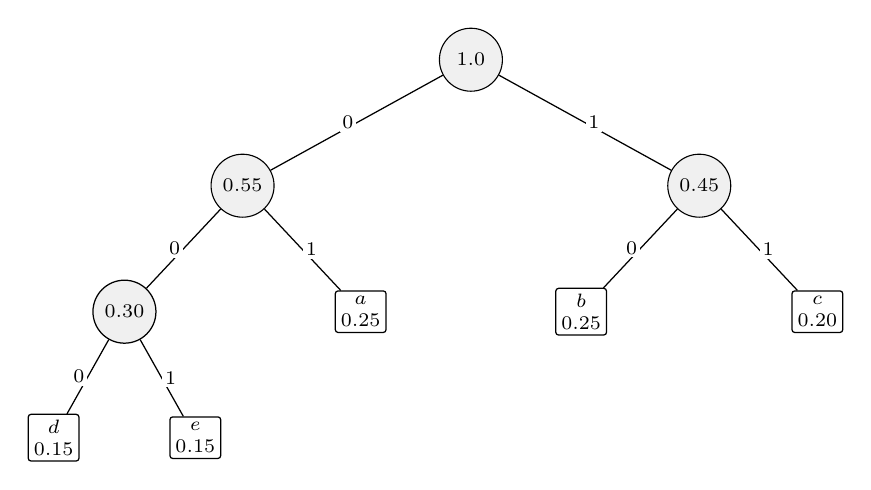
\begin{tikzpicture}[
    level distance=16mm,
    level 1/.style={sibling distance=58mm},
    level 2/.style={sibling distance=30mm},
    level 3/.style={sibling distance=18mm},
    edge from parent/.style={draw, line width=0.45pt},
    every node/.style={font=\scriptsize, align=center},
    edge label/.style={font=\scriptsize, inner sep=1pt, fill=white},
    internal/.style={circle, draw, fill=black!6, minimum size=8mm, inner sep=1pt},
    leaf/.style={rectangle, draw, rounded corners=1pt, fill=white, inner sep=2pt}
]
% Albero di Huffman per la sorgente:
% a,b,c,d,e con probabilita' 0.25, 0.25, 0.20, 0.15, 0.15.
\node[internal] {$1.0$}
    child {
        node[internal] {$0.55$}
        child {
            node[internal] {$0.30$}
            child {
                node[leaf] {$d$\\$0.15$}
                edge from parent node[edge label, left] {$0$}
            }
            child {
                node[leaf] {$e$\\$0.15$}
                edge from parent node[edge label, right] {$1$}
            }
            edge from parent node[edge label, left] {$0$}
        }
        child {
            node[leaf] {$a$\\$0.25$}
            edge from parent node[edge label, right] {$1$}
        }
        edge from parent node[edge label, left] {$0$}
    }
    child {
        node[internal] {$0.45$}
        child {
            node[leaf] {$b$\\$0.25$}
            edge from parent node[edge label, left] {$0$}
        }
        child {
            node[leaf] {$c$\\$0.20$}
            edge from parent node[edge label, right] {$1$}
        }
        edge from parent node[edge label, right] {$1$}
    };
\end{tikzpicture}
\end{document}
